\documentclass{article}

\usepackage[english, russian]{babel}
\usepackage{geometry}
\usepackage{graphicx}
\usepackage{listings}
\usepackage{xcolor}
\usepackage[14pt]{extsizes}
\usepackage{amsmath}
\usepackage{setspace}
\usepackage{multirow}
\usepackage{tocloft}
\usepackage{indentfirst} 
\usepackage{lipsum}
\usepackage{caption}
\usepackage{cmap}
\usepackage[utf8]{inputenc}
\usepackage[T2A]{fontenc}

\captionsetup[figure]{name={Рисунок},labelsep=endash}
\captionsetup[table]{singlelinecheck=false, labelsep=endash}

\renewcommand{\cftsecleader}{\cftdotfill{\cftdotsep}}
\geometry{pdftex, left = 3cm, right = 1cm	, top = 2cm, bottom = 2cm}
\onehalfspacing

\setlength{\parindent}{1,25cm}
\lstdefinestyle{lst}{
	basicstyle=\footnotesize\ttfamily,
	frame=single,
	tabsize=4,	
	breaklines=true
}

\DeclareCaptionLabelSeparator{line}{\ --\ }
\DeclareCaptionFont{white}{\color{white}}
\DeclareCaptionFormat{listing}{\colorbox[cmyk]{0.43,0.35,0.35,0.01}{\parbox{\textwidth}{\hspace{15pt}#1#2#3}}}
\captionsetup[lstlisting]{
	singlelinecheck=false,
	labelsep=line
}

\begin{document}
\begin{titlepage}
	\newgeometry{pdftex, left=2cm, right=2cm, top=2.5cm, bottom=2.5cm}
	\fontsize{12pt}{12pt}\selectfont
	\noindent\begin{tabular}{|c|c|}	\hline
	\noindent\begin{minipage}{0.15\textwidth}
		
\includegraphics[width=\linewidth]{tools/logo.png}
	\end{minipage} &
	\noindent\begin{minipage}{0.85\textwidth}\centering
		\textbf{\newline Министерство науки и высшего образования Российской Федерации}\\
		\textbf{Федеральное государственное бюджетное образовательное учреждение высшего образования}\\
		\textbf{«Московский государственный технический университет имени Н.Э.~Баумана}\\
		\textbf{(национальный исследовательский университет)»}\\
		\textbf{(МГТУ им. Н.Э.~Баумана)}
	\end{minipage} \\
	\hline	\end{tabular}\newline\newline\newline
	\noindent ФАКУЛЬТЕТ \underline{«Информатика и системы управления»} \newline\newline
	\noindent КАФЕДРА \underline{«Программное обеспечение ЭВМ и информационные технологии»}\newline\newline\newline\newline\newline\newline

	\noindent\begin{minipage}{1.0\textwidth}\centering
		\Large\textbf{   ~~~ Лабораторная работа №2}\newline
		\textbf{по дисциплине «Архитектура ЭВМ»}\newline\newline\newline\newline\newline
	\end{minipage}

	\noindent\textbf{Тема} \underline{Изучение принципов работы микропроцессорного ядра RISC-V}
\newline\newline
	\textbf{Студент} \underline{Тузов Даниил Александрович}\newline\newline
	\textbf{Группа} \underline{ИУ7-52Б}\newline\newline
	\textbf{Преподаватель} \underline{Калитвенец Максим, Попов А.Ю.}
	
	\begin{center}
		\vfill
		Москва, \the\year ~г.
	\end{center}
	\restoregeometry
	\clearpage
\end{titlepage}

\section{Введение}
Основной \textbf{целью} работы является ознакомление с принципами функционирования, построения и особенностями 
архитектуры суперскалярных конвейерных микропроцессоров. Дополнительной \textbf{целью} работы является знакомство с 
принципами проектирования и верификации сложных цифровых устройств с использованием языка описания аппаратуры 
SystemVerilog и ПЛИС.

Для достижения поставленных целей в настоящей лабораторной работе используется синтезируемое описание 
микропроцессорного ядра Taiga, реализующего систему команд RV32I семейства RISC-V. Данное описание выполнено на языке 
описания аппаратуры SystemVerilog.

В ходе лабораторной работы используется средство моделирования MentorGraphics Modelsim для моделирования работы 
исследуемого микропроцессора в процессе выполнения программы и наблюдения формы внутренних сигналов.

\section{Задание 1}
\subsection{Исходный текст исследуемой программы}
\begin{lstlisting}[style=lst, caption=Исходный текст исследуемой программы]
.section .text
        .globl _start;
        len = 9 
        enroll = 2 
        elem_sz = 4
_start:
        la x1, _x
        addi x20, x1, elem_sz*len
        lw x31, 0(x1)
        addi x1, x1, elem_sz*1
lp:
        lw x2, 0(x1)    #!
        lw x3, 4(x1)
        bltu x2, x31, lt1
        add x31, x0, x2
lt1:    bltu x3, x31, lt2
        add x31, x0, x3
lt2:
        add x1, x1, elem_sz*enroll
        bne x1, x20, lp
lp2: j lp2
        .section .data
_x:     .4byte 0x1
        .4byte 0x2
        .4byte 0x3
        .4byte 0x4
        .4byte 0x8
        .4byte 0x6
        .4byte 0x7
        .4byte 0x5
        .4byte 0x4
\end{lstlisting}

\subsection{Дизассемблированный листинг}
\begin{lstlisting}[style=lst, caption=Дизассемблированный листинг программы]
Disassembly of section .text:
80000000 <_start>:
80000000:  00000097            auipc  x1,0x0
80000004:  03808093            addi  x1,x1,56 # 80000038 <_x>
80000008:  02408a13            addi  x20,x1,36
8000000c:  0000af83            lw  x31,0(x1)
80000010:  00408093            addi  x1,x1,4
80000014 <lp>:
80000014:  0000a103            lw  x2,0(x1)
80000018:  0040a183            lw  x3,4(x1)
8000001c:  00808093            addi  x1,x1,8
80000020:  01f16463            bltu  x2,x31,80000028 <lt1>
80000024:  00200fb3            add  x31,x0,x2
80000028 <lt1>:
80000028:  01f1e463            bltu  x3,x31,80000030 <lt2>
8000002c:  00300fb3            add  x31,x0,x3
80000030 <lt2>:
80000030:  ff4092e3            bne  x1,x20,80000014 <lp>
80000034 <lp2>:
80000034:  0000006f            jal  x0,80000034 <lp2>
Disassembly of section .data:
80000038 <_x>:
80000038:  0001                  .insn  2, 0x0001
8000003a:  0000                  .insn  2, 0x
8000003c:  0002                  .insn  2, 0x0002
8000003e:  0000                  .insn  2, 0x
80000040:  00000003            lb  x0,0(x0) # 0 <enroll-0x2>
80000044:  0004                  .insn  2, 0x0004
80000046:  0000                  .insn  2, 0x
80000048:  0008                  .insn  2, 0x0008
8000004a:  0000                  .insn  2, 0x
8000004c:  0006                  .insn  2, 0x0006
8000004e:  0000                  .insn  2, 0x
80000050:  00000007            .insn  4, 0x0007
80000054:  0005                  .insn  2, 0x0005
80000056:  0000                  .insn  2, 0x
80000058:  0004                  .insn  2, 0x0004
\end{lstlisting}

\subsection{Псевдокод, поясняющий работу программы}
\begin{lstlisting}[style=lst, caption=Псевдокод]
#define len 9
#define enroll 2
#define elem_sz 4
unsigned _x[] = { 1, 2, 3, 4, 8, 6, 7, 5, 4 };
void _start() {
    unsigned *x1 = _x; // la x1, _x
    unsigned *x20 = x1 + len; // addi x20, x1, elem_sz*len
    unsigned x31 = x1[0]; // lw x31, 0(x1)
    x1 += 1; // addi x1, x1, elem_sz*1
    do {
        // lp
        unsigned x2 = x1[0]; // lw x2, 0(x1)
        unsigned x3 = x1[1]; // lw x3, 4(x1)
        if (x2 < x31) { // bltu x2, x31, lt1
        else
            x31 = x2; // add x31, x0, x2
        // lt1
        if (x3 < x31) // bltu x3, x31, lt2
        else
            x31 = x3; // add x31, x0, x3
        // lt2
        x1 += enroll; // add x1, x1, elem_sz*enroll
    } while (x1 != x20); // bne x1, x20, lp
    for (;;); // lp2: j lp2
}
\end{lstlisting}

\clearpage\section{Задание 2}
\begin{figure}[h]
	\centering
	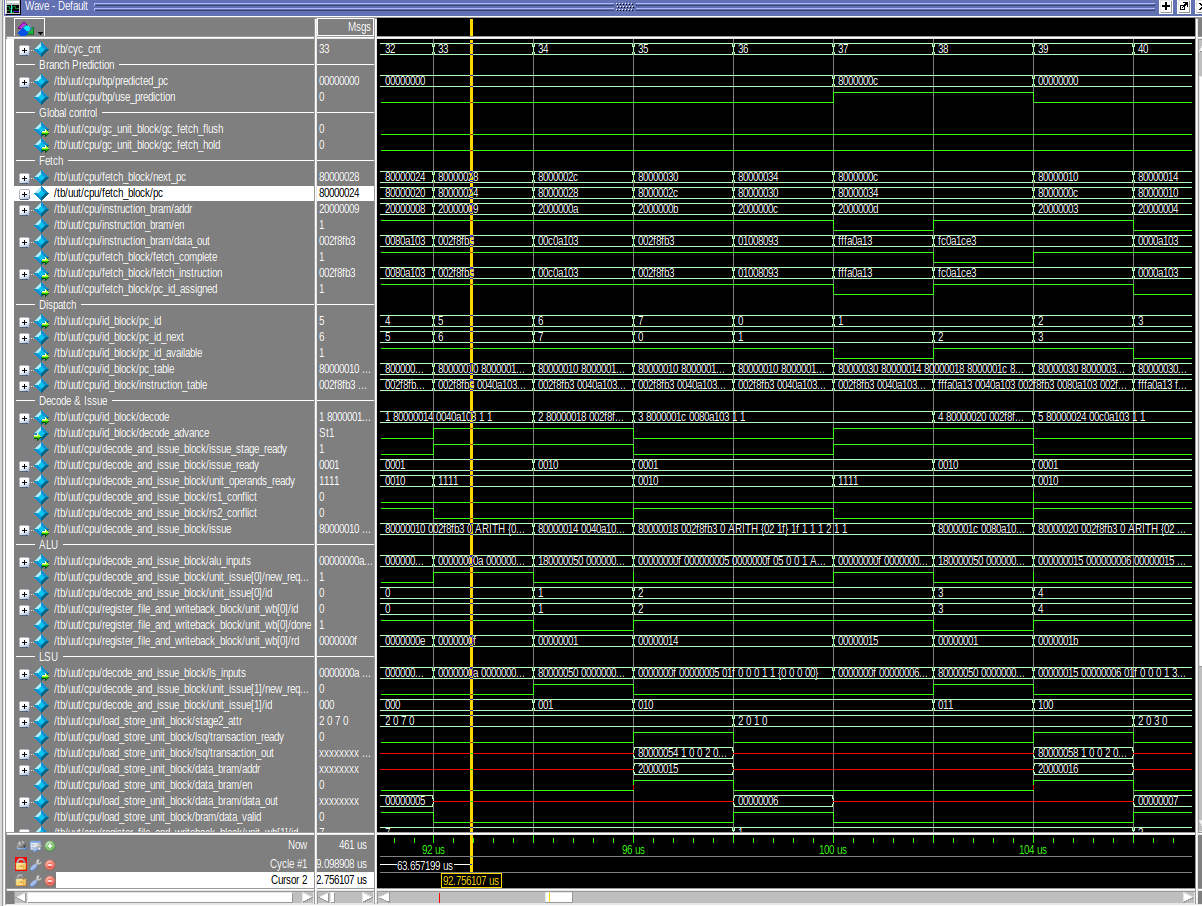
\includegraphics[scale=0.4]{tools/task2.png}
	\caption{Стадии выборки и диспетчеризации}
\end{figure}

\clearpage\section{Задание 3}
\begin{figure}[h]
	\centering
	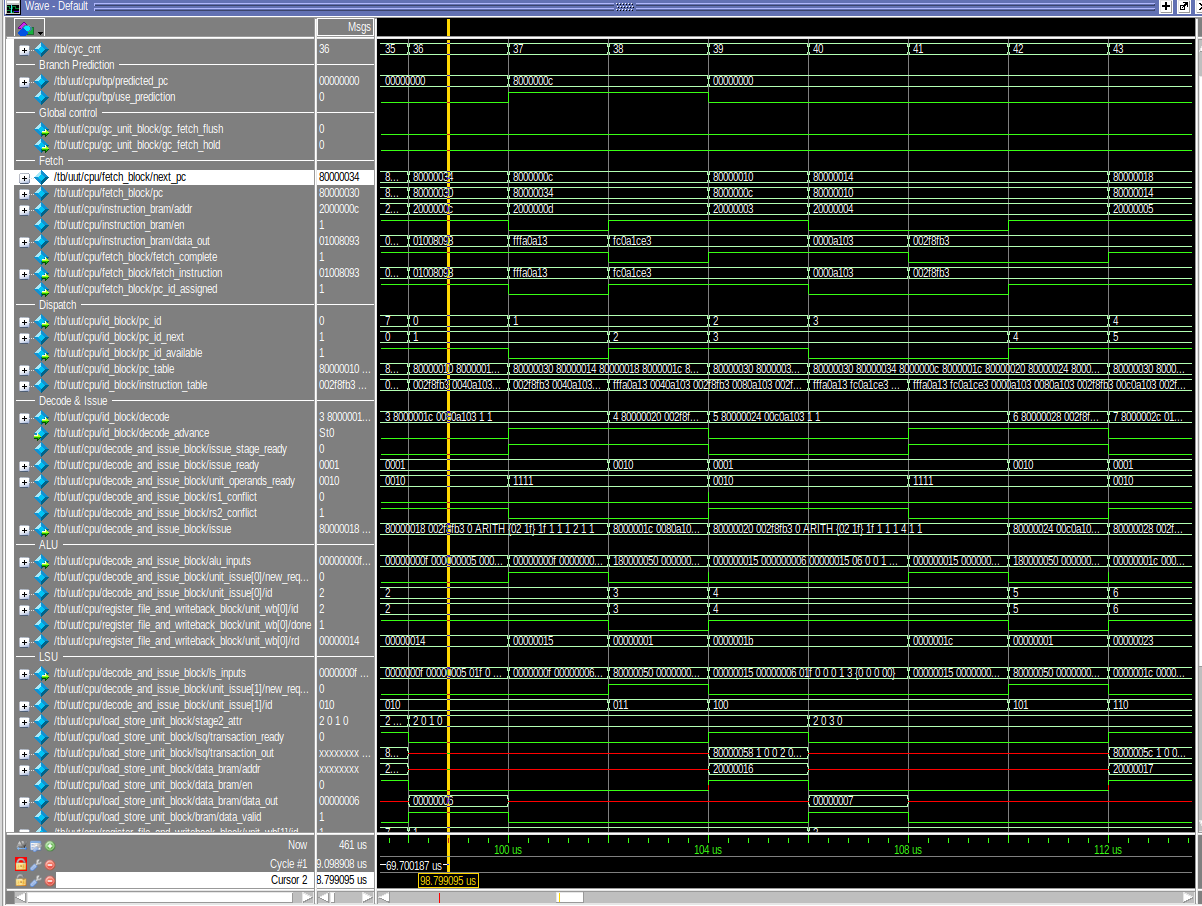
\includegraphics[scale=0.4]{tools/task3.png}
	\caption{Стадии декодирования и планирования}
\end{figure}

\clearpage\section{Задание 4}
\begin{figure}[h]
	\centering
	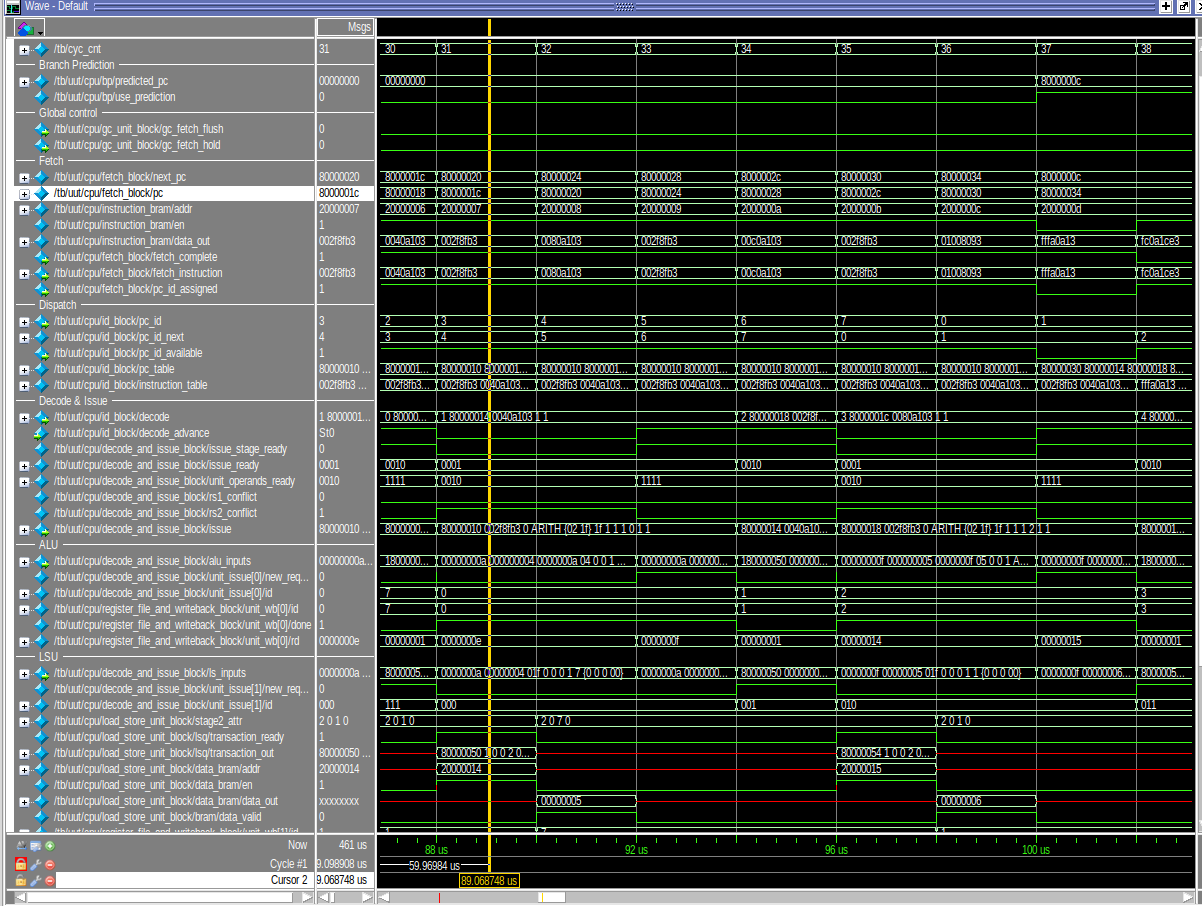
\includegraphics[scale=0.4]{tools/task4.png}
	\caption{Непосредственное выполнение комманды}
\end{figure}

\clearpage\section{Задание 5}
\subsection{Место, отмеченное решеткой}
\begin{figure}[h]
	\centering
	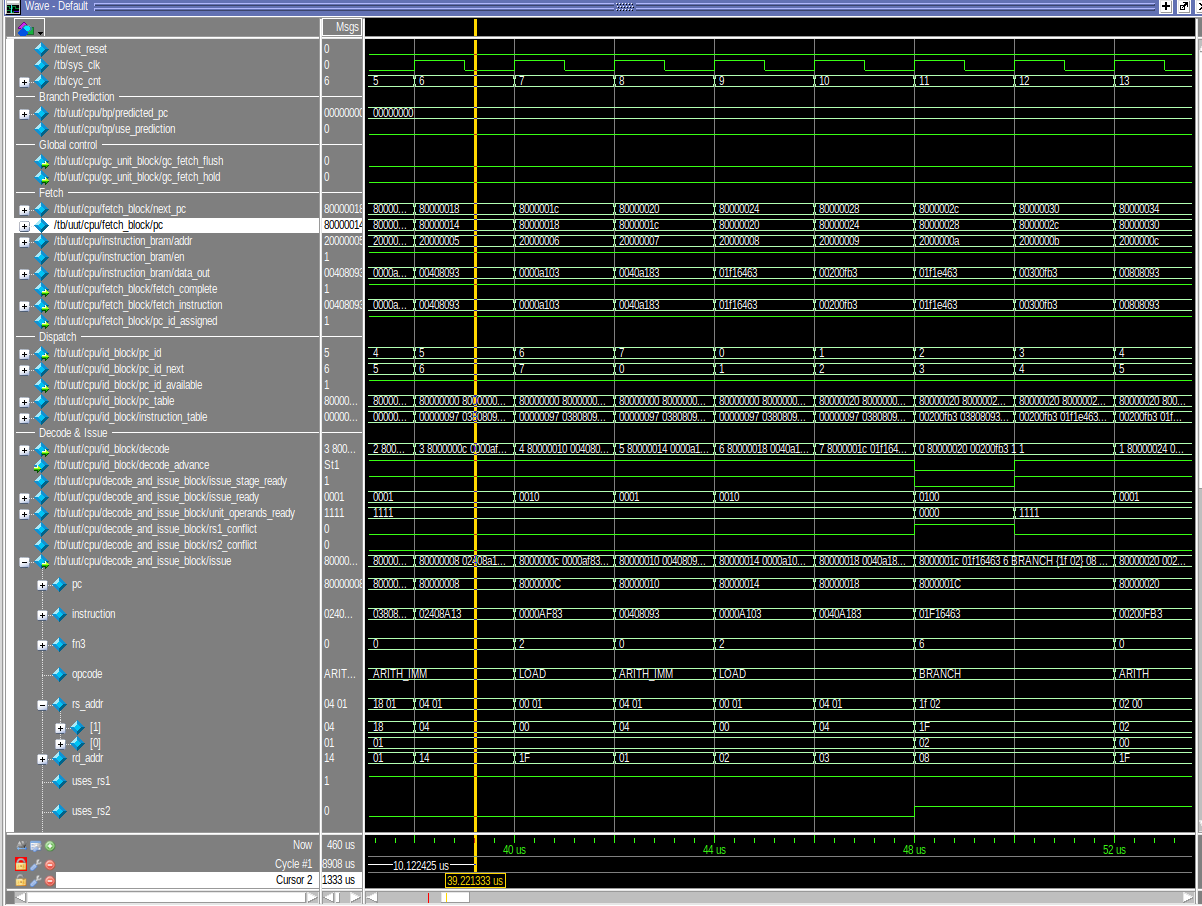
\includegraphics[scale=0.4]{tools/task5_1.png}
	\caption{Первая итерация команды, отмеченной \#}
\end{figure}

\begin{figure}[h]
	\centering
	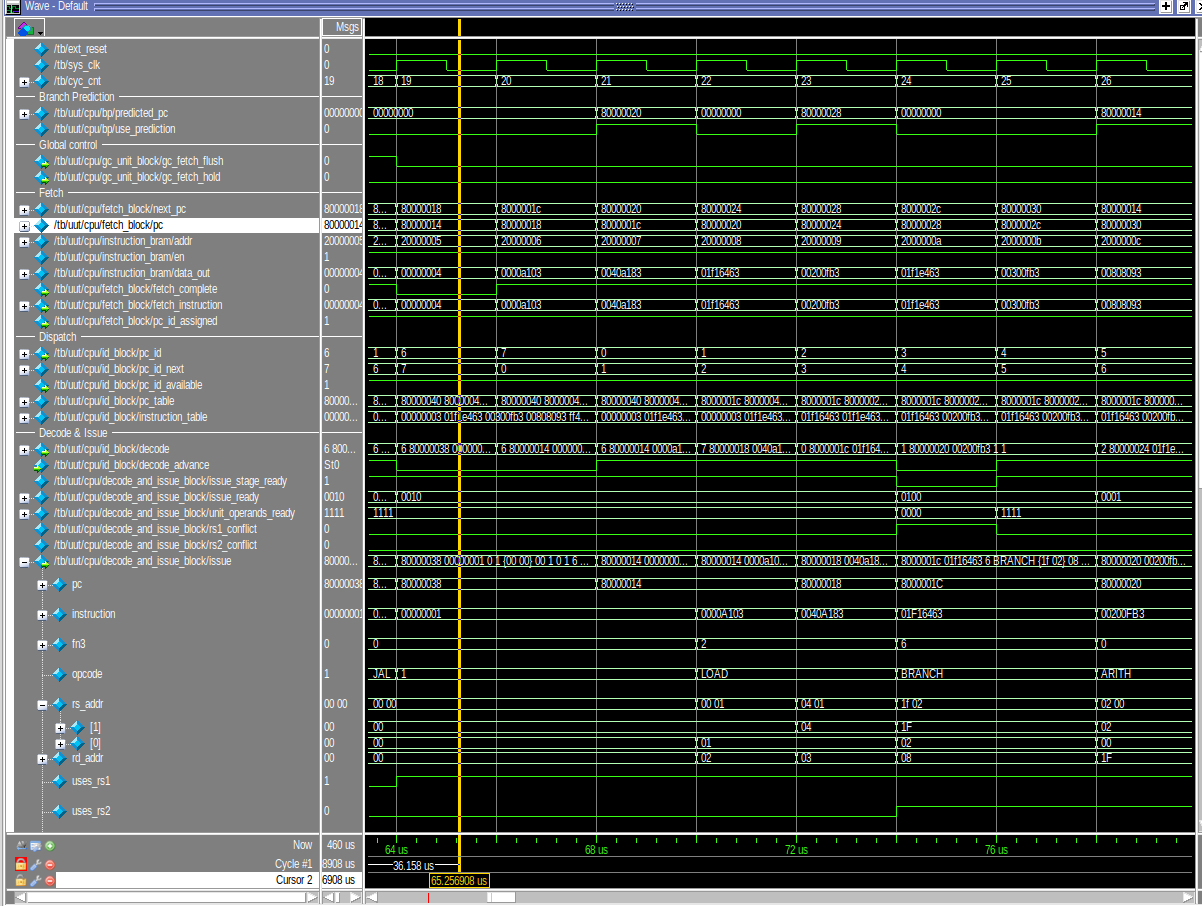
\includegraphics[scale=0.4]{tools/task5_2.png}
	\caption{Вторая итерация команды, отмеченной \#}
\end{figure}

\clearpage\subsection{Трасса исходной программы}
\begin{figure}[h]
	\centering
	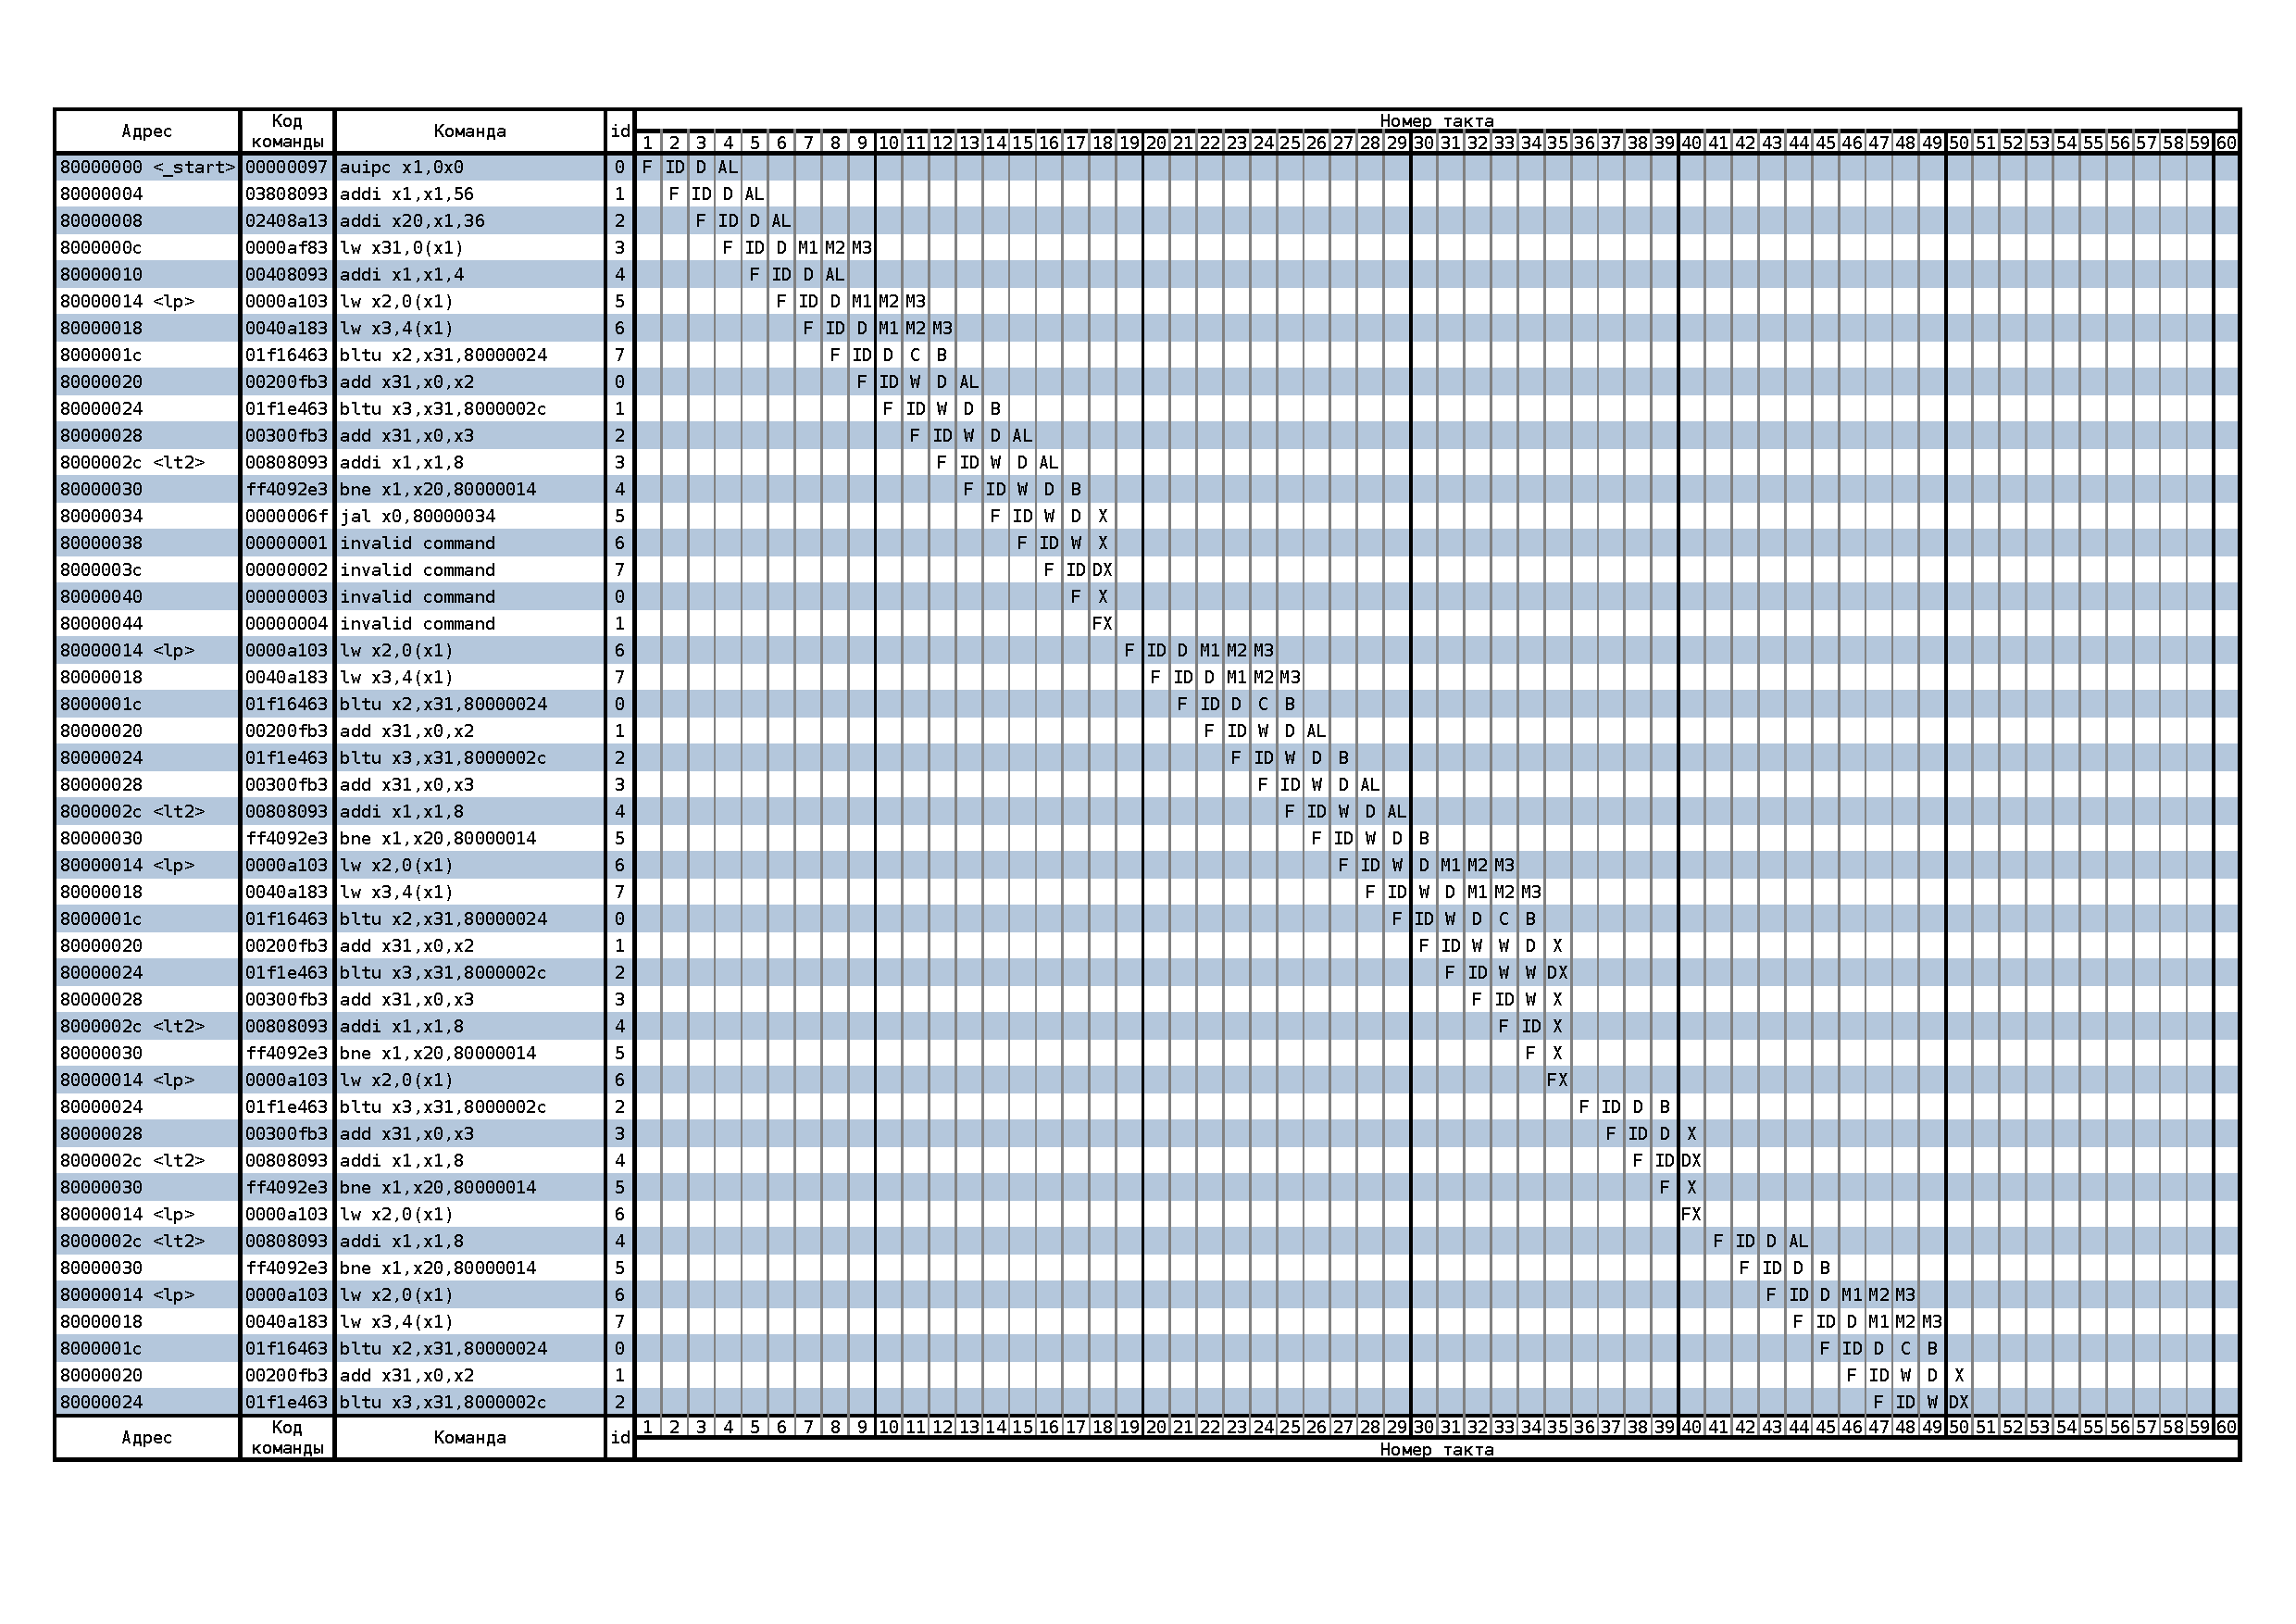
\includegraphics[scale=0.4]{tools/line.pdf}
          \caption{Трасса выполнения неоптимизированной программы}
\end{figure}

Конфликты возникают из-за того, что происходит обращение к регистру, запись в который ещё не была завершена (регистр x2).

Cтрока x1 += enroll (add x1, x1, elem\_sz*enroll) будет выполнена вне зависимости от предшествующих условных переходов, а 
также значение регистра x1 не используется после строки lw x3, 4(x1) в пределах выполнения тела цикла.

Следовательно, если поместить строку add x1, x1, slem\_sz*enroll сразу после lw x3, 4(x1), это не повлияет на результат 
выполнения программы, зато даст дополнительную задержку в один такт между загрузкой значения в x2 и чтением из него, что 
позволит устранить конфликты.

\clearpage\subsection{Исходной текст оптимизированной программы}
\begin{lstlisting}[style=lst, caption=Исходный текст оптимизированной программы]
.section .text
        .globl _start;
        len = 9
        enroll = 2
        elem_sz = 4 
_start:
        la x1, _x
        addi x20, x1, elem_sz*len
        lw x31, 0(x1)
        addi x1, x1, elem_sz*1
lp:
        lw x2, 0(x1) #!
        lw x3, 4(x1)
        add x1, x1, elem_sz*enroll
        bltu x2, x31, lt1
        add x31, x0, x2
lt1:    bltu x3, x31, lt2
        add x31, x0, x3
lt2:
        bne x1, x20, lp
lp2: j lp2
        .section .data
_x:     .4byte 0x1
        .4byte 0x2
        .4byte 0x3
        .4byte 0x4
        .4byte 0x8
        .4byte 0x6
        .4byte 0x7
        .4byte 0x5
        .4byte 0x4
\end{lstlisting}

\clearpage\subsection{Дизассемблированный листинг оптимизированной программы}
\begin{lstlisting}[style=lst, caption=Дизассемблированный листинг оптимизированной программы]
Disassembly of section .text:
80000000 <_start>:
80000000:  00000097            auipc  x1,0x0
80000004:  03808093            addi  x1,x1,56 # 80000038 <_x>
80000008:  02408a13            addi  x20,x1,36
8000000c:  0000af83            lw  x31,0(x1)
80000010:  00408093            addi  x1,x1,4
80000014 <lp>:
80000014:  0000a103            lw  x2,0(x1)
80000018:  0040a183            lw  x3,4(x1)
8000001c:  01f16463            bltu  x2,x31,80000024 <lt1>
80000020:  00200fb3            add  x31,x0,x2
80000024 <lt1>:
80000024:  01f1e463            bltu  x3,x31,8000002c <lt2>
80000028:  00300fb3            add  x31,x0,x3
8000002c <lt2>:
8000002c:  00808093            addi  x1,x1,8
80000030:  ff4092e3            bne  x1,x20,80000014 <lp>
80000034 <lp2>:
80000034:  0000006f            jal  x0,80000034 <lp2>
Disassembly of section .data:
80000038 <_x>:
80000038:  0001                  .insn  2, 0x0001
8000003a:  0000                  .insn  2, 0x
8000003c:  0002                  .insn  2, 0x0002
8000003e:  0000                  .insn  2, 0x
80000040:  00000003            lb  x0,0(x0) # 0 <enroll-0x2>
80000044:  0004                  .insn  2, 0x0004
80000046:  0000                  .insn  2, 0x
80000048:  0008                  .insn  2, 0x0008
8000004a:  0000                  .insn  2, 0x
8000004c:  0006                  .insn  2, 0x0006
8000004e:  0000                  .insn  2, 0x
80000050:  00000007            .insn  4, 0x0007
80000054:  0005                  .insn  2, 0x0005
80000056:  0000                  .insn  2, 0x
80000058:  0004                  .insn  2, 0x0004
\end{lstlisting}

\clearpage\subsection{Трасса оптимизированной программы}
\begin{figure}[h]
	\centering
	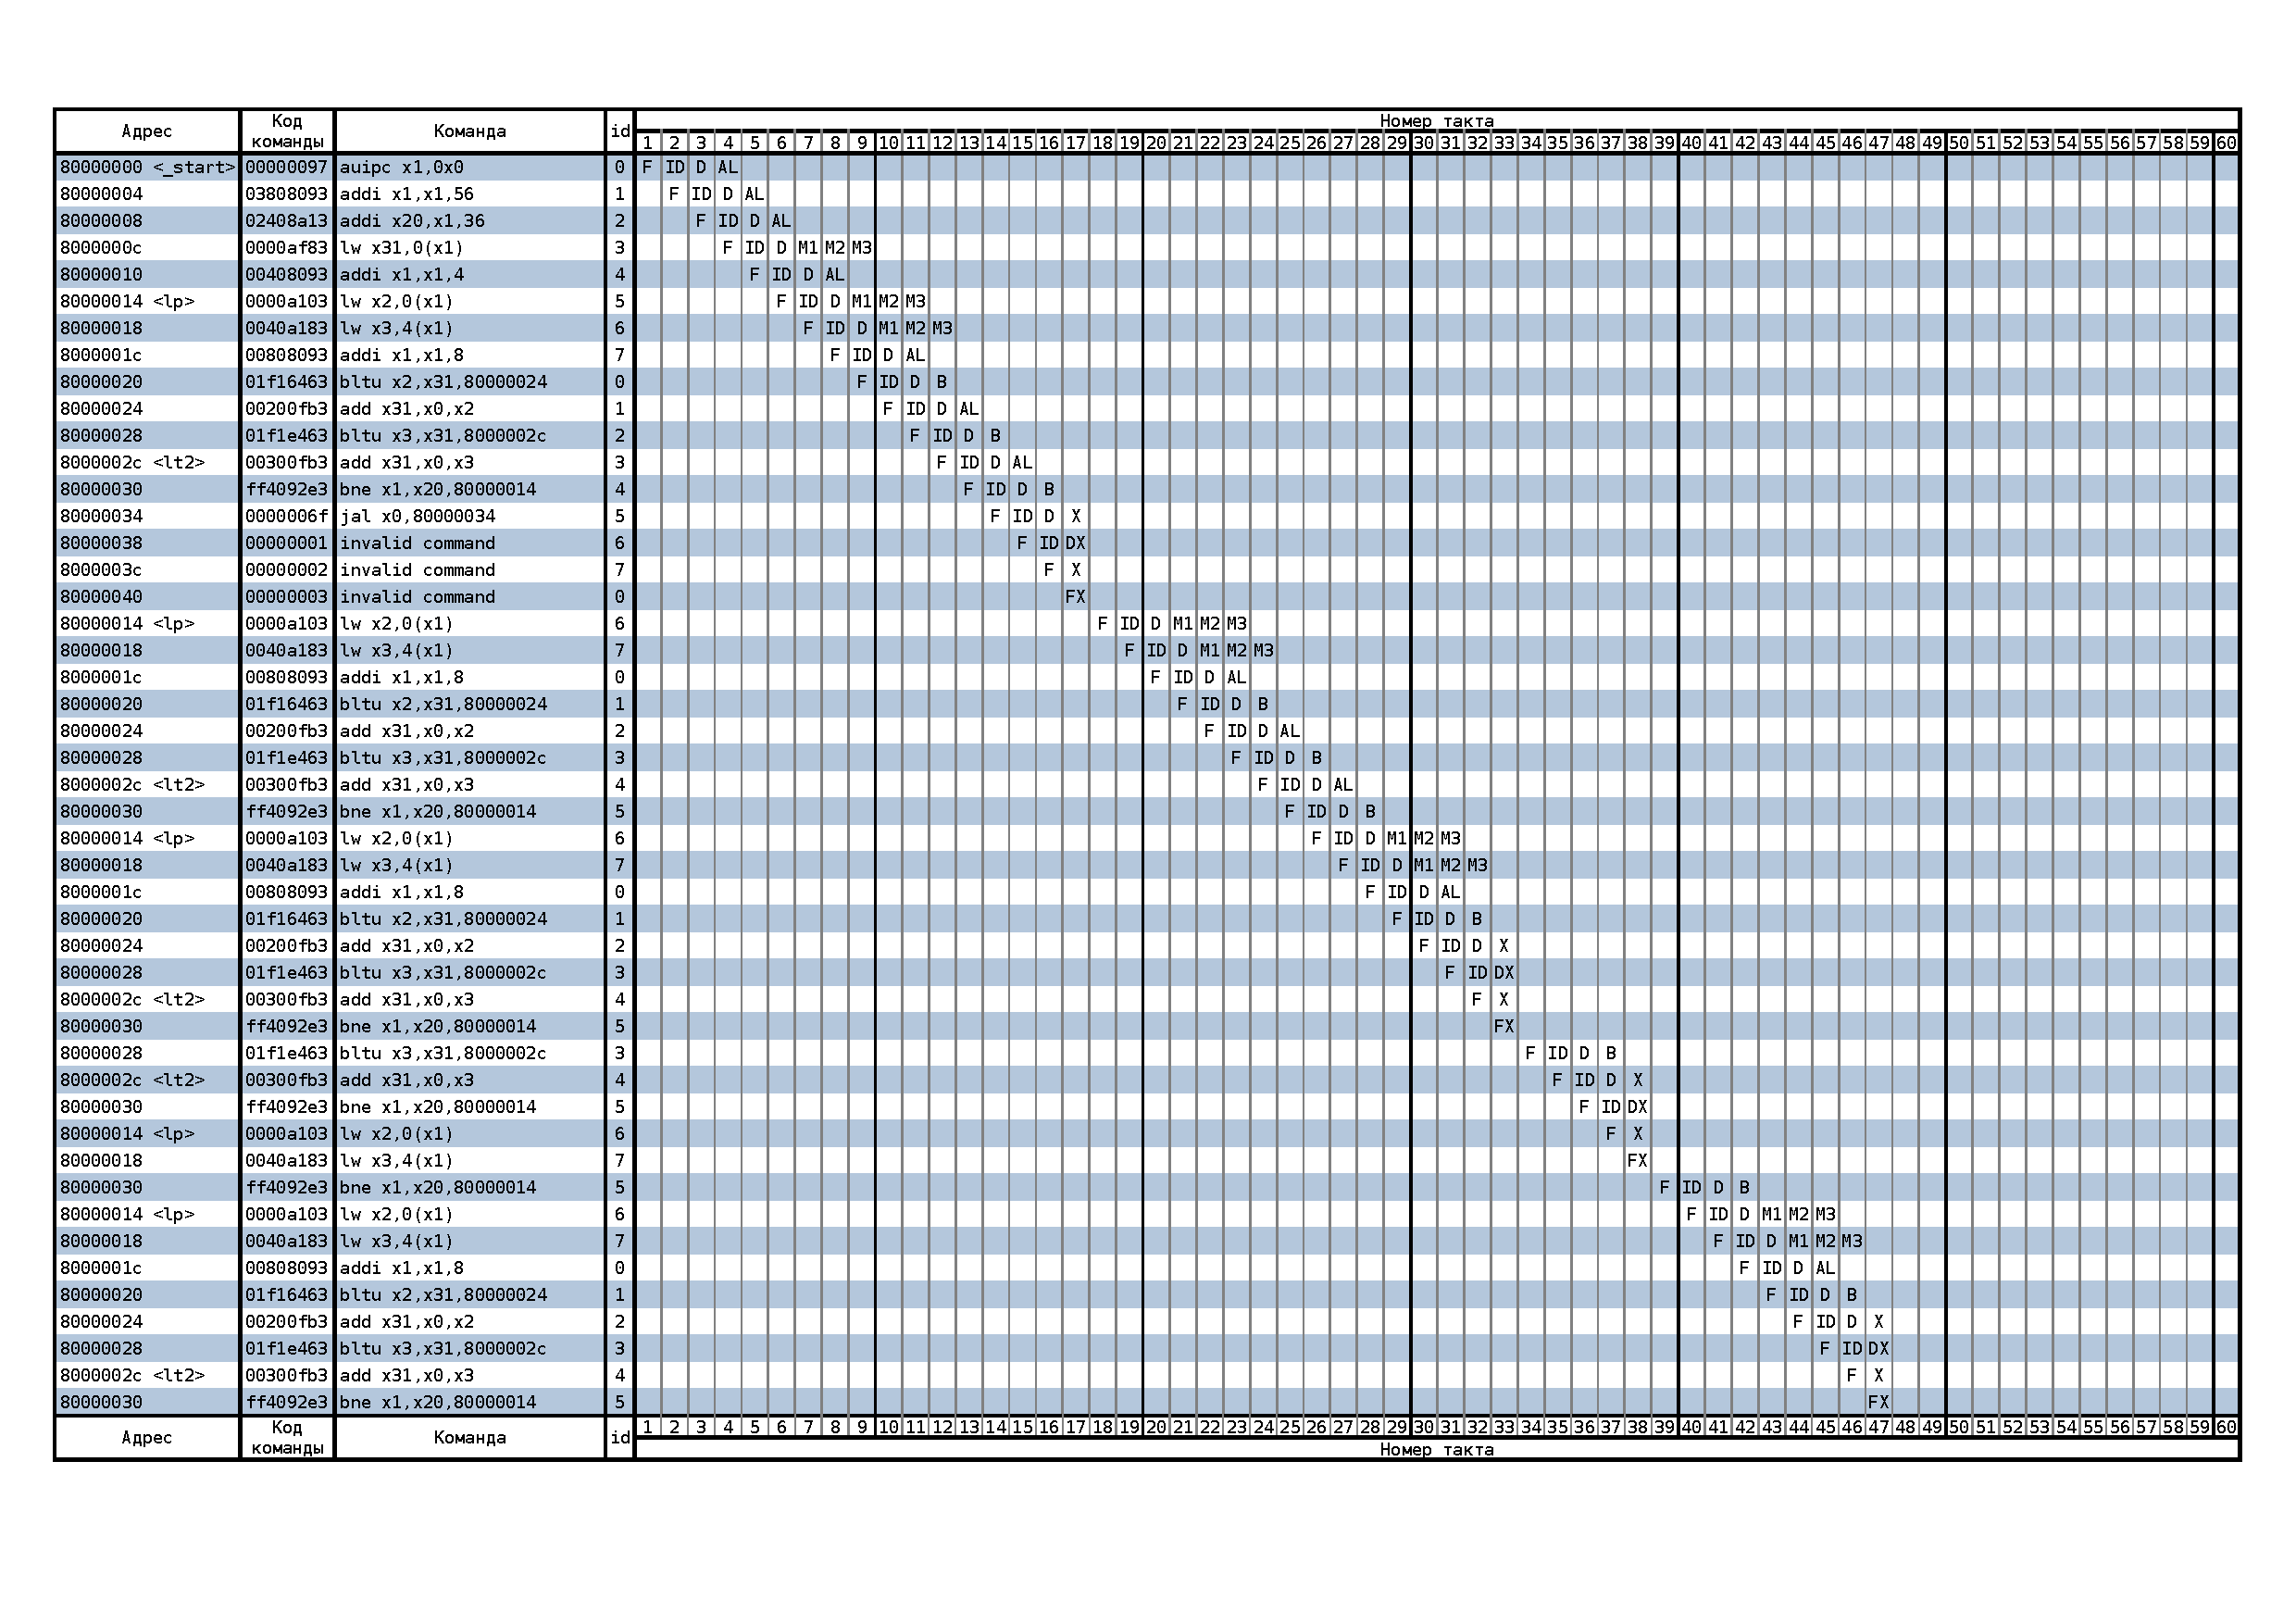
\includegraphics[scale=0.4]{tools/line_opt.pdf}
          \caption{Трасса выполнения оптимизированной программы}
\end{figure}

Можно заметить, что конфликтов больше нет, а трасса стала на два такта короче (на 4\%).

\section{Вывод}
В результате данной работы были изучены принципы функционирования, построения и особенности архитектуры 
суперскалярных конвейерных микропроцессоров.

На основе изученных материалов удалось оптимизировать программу.
\end{document}